\documentclass{article}
\usepackage[utf8]{inputenc}

\usepackage{amssymb}
\usepackage{amsmath}
\usepackage{float}

\title{Time Series Project 1}
\author{Stefan Eng and Franz Hartleitner}
\date{April 2019}

\usepackage{natbib}
\usepackage{graphicx}

\begin{document}

\maketitle

\section*{Problem 1}

\begin{figure}[H]
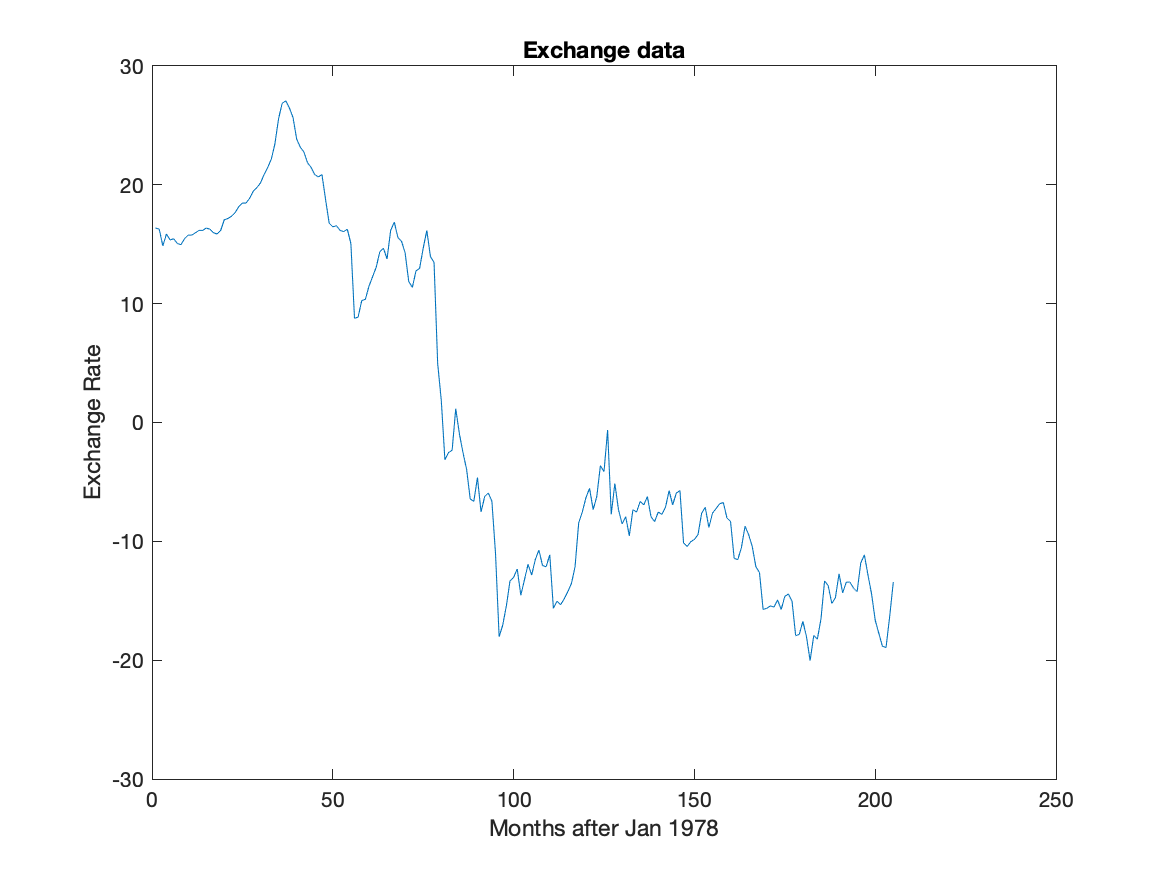
\includegraphics[width=10cm]{plots/exchangedata.png}
\centering
\caption{Monthly observations of the Australian Trade Weighted Index}
\label{fig:exchangerate}
\end{figure}

In Figure \ref{fig:exchangerate} we we can see the the monthly observations of the Australian Trade Weighted Index.
From this graph it does not appear to be a stationary process.
For an lag set to say $h = 10$, if we look at the relation between $t = 25$ and $t = 75$, we see that the covariance is positive between $X_{25}$ and $X_{35}$ and fairly strongly negatively correlated between $X_{75}$ and $X_{85}$.
This shows informally that we are probably not dealing with a stationary time series as we would expect the covariance of $\gamma_{X}(t + h, t)$ not to depend on $t$.

\begin{figure}[H]
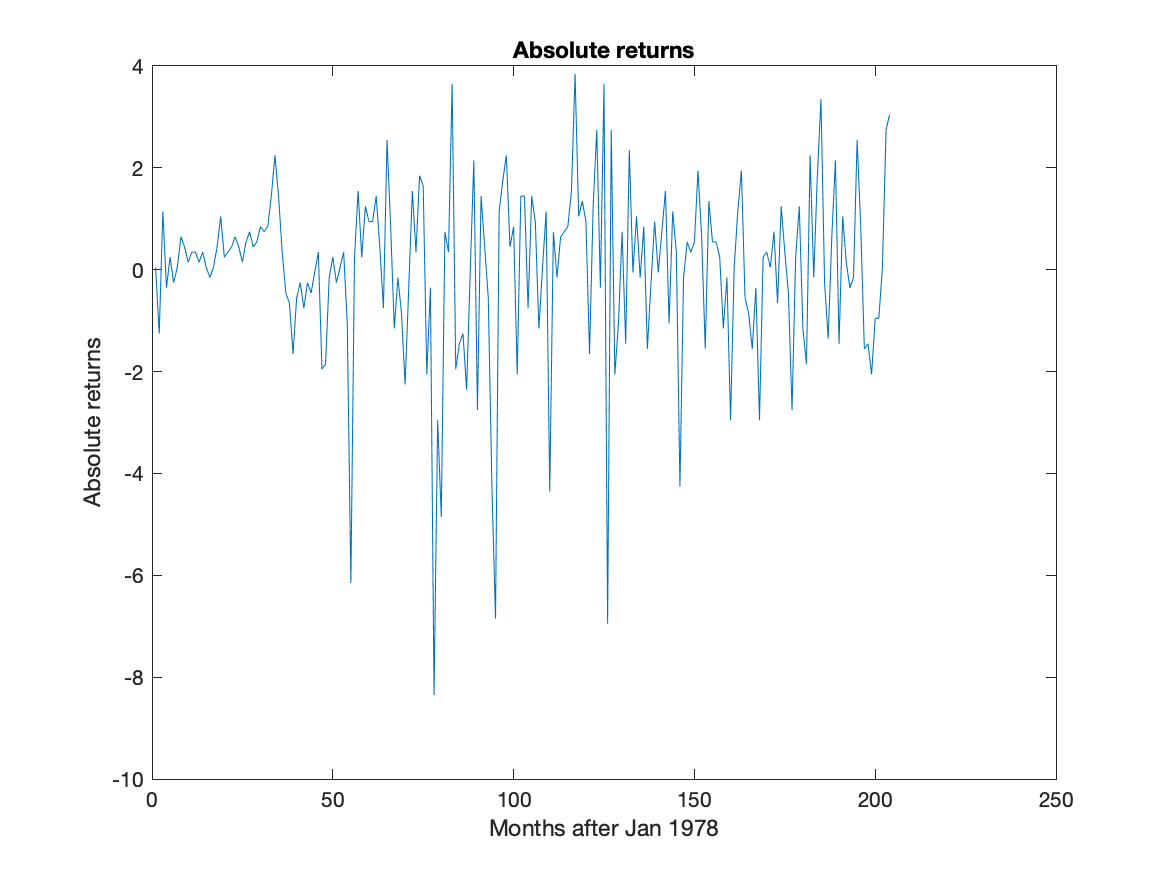
\includegraphics[width=10cm]{plots/abs_returns.png}
\centering
\caption{Absolute returns $Y_t = X_{t + 1} - X_{t}$}
\label{fig:absreturns}
\end{figure}

\begin{figure}[H]
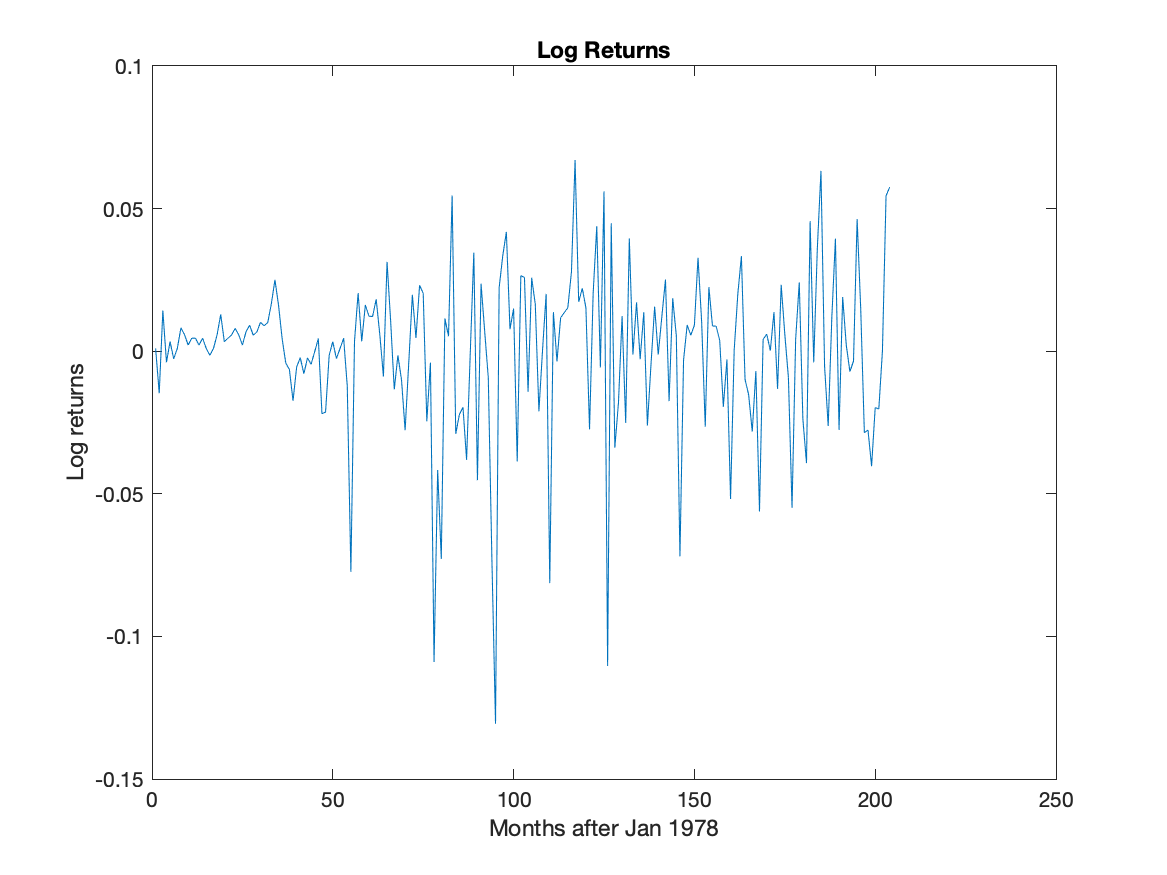
\includegraphics[width=10cm]{plots/log_returns.png}
\centering
\caption{Log returns $Z_t = \log(X_{t + 1}) - \log(X_{t})$}
\label{fig:logreturns}
\end{figure}

For both the absolute returns in Figure \ref{fig:absreturns} and the log returns in Figure \ref{fig:logreturns} it appears that the processes could be stationary.
There do not seem to be any pairs of points where the covariance of $X_{t + h}$ and $X_{t}$ would be dependent on the value of $t$.
The range of $t$ from $0 \leq t 40$ does appear slightly different from the rest of the series but not enough for us to think it would not be stationary.
Overall both series actually do not look like they have very much correlation at all between which could be an indication of independent and identically distributed time series.

\section*{Problem 2}
To test whether the series are iid or not we use the Ljung-Box test that compares the test statistic
$$
\lambda = n (n + 2) \sum_{i = 1}^h \frac{\hat{\rho}(i)^2}{n - i}
$$
Which has a $\chi^2_{h}$ distribution under the null hypothesis (that the data comes from and iid distribution
We want to test with $h = 20$ and $\alpha = 0.05$ so we compare $\lambda$ again the critical value, $\chi^2_{1-\alpha,h}$. That is, we reject the null hypothesis if
$$
\lambda > \chi^2_{.95,20} = 31.41
$$

For the standardized exchange rate data we found that $\lambda_1 = 3005$ which has a $p$-value of essentially 0. We can reject the null hypothesis and concluded that the exchange rate data is not iid.

For the absolute returns, we found that $\lambda_2 = 29.09$. That corresponds with a p-value of $0.086 > 0.05$. Here we fail to reject the null hypothesis (but we are fairly close to .05). There is some evidence to support the claim that the absolute returns are iid.

The log returns have a test statistic $\lambda_3 = 23.19$ which has a p-value of 0.279. Here we fail to reject the null hypothesis as well which is consistent with the log returns being iid.

The ACF are plotted in Figures \ref{fig:acf_exchange}, \ref{fig:acf_abs}, and \ref{fig:acf_log}.
The dashed lines represent $\pm 1.96 / \sqrt{n}$.
If the data was an iid sequence we would expect 95\% (approximately 10 point) of the sample to fall within these bounds \cite{bd}.
We see that almost all the points are within these bounds.
This is consistent with out findings in the Ljung-Box test.
We can see a steady decrease in the ACF for the exchange data which indicates that we could probably predict these values better than the absolute returns and log returns.

\begin{figure}[H]
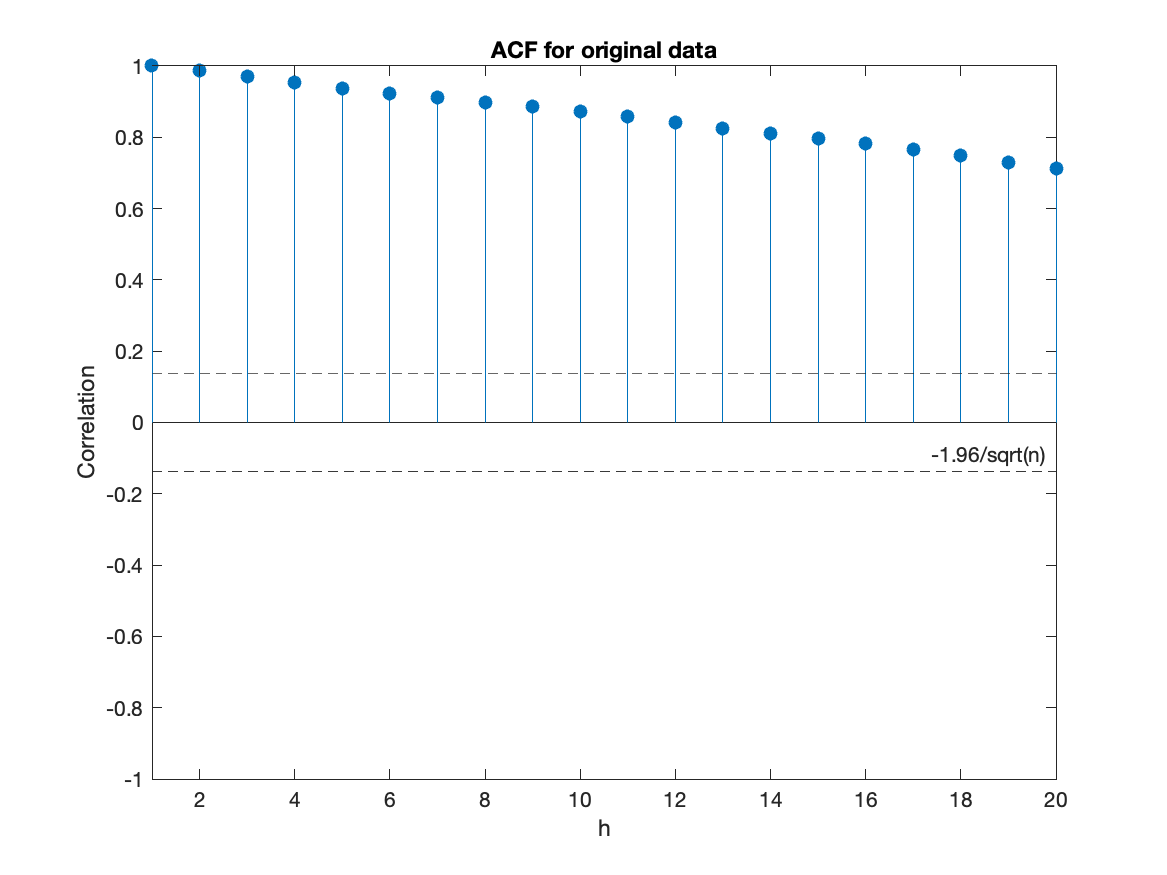
\includegraphics[width=10cm]{plots/acf_exchange.png}
\centering
\caption{ACF for Exchange Data $h = 0,\ldots, 20$}
\label{fig:acf_exchange}
\end{figure}

\begin{figure}[H]
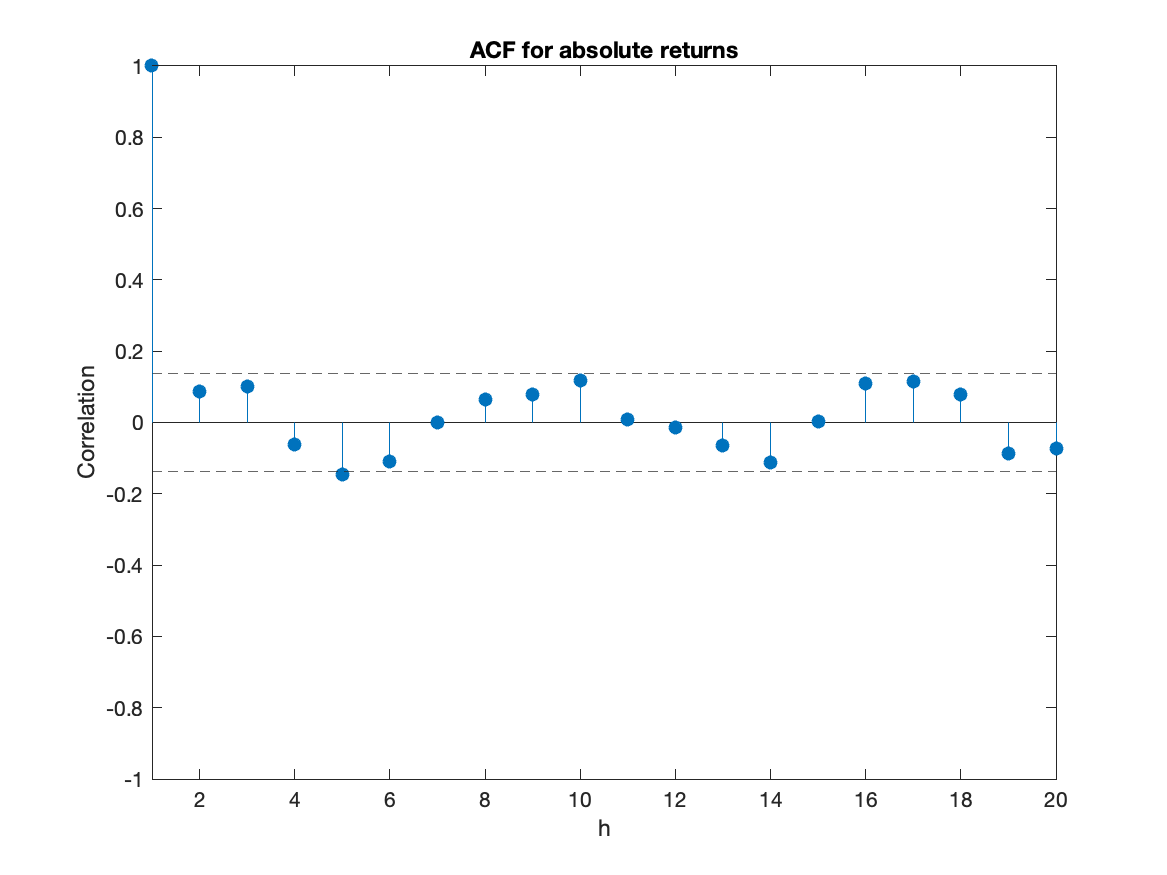
\includegraphics[width=10cm]{plots/acf_abs_returns.png}
\centering
\caption{ACF for Absolute Returns $h = 0,\ldots, 20$}
\label{fig:acf_abs}
\end{figure}

\begin{figure}[H]
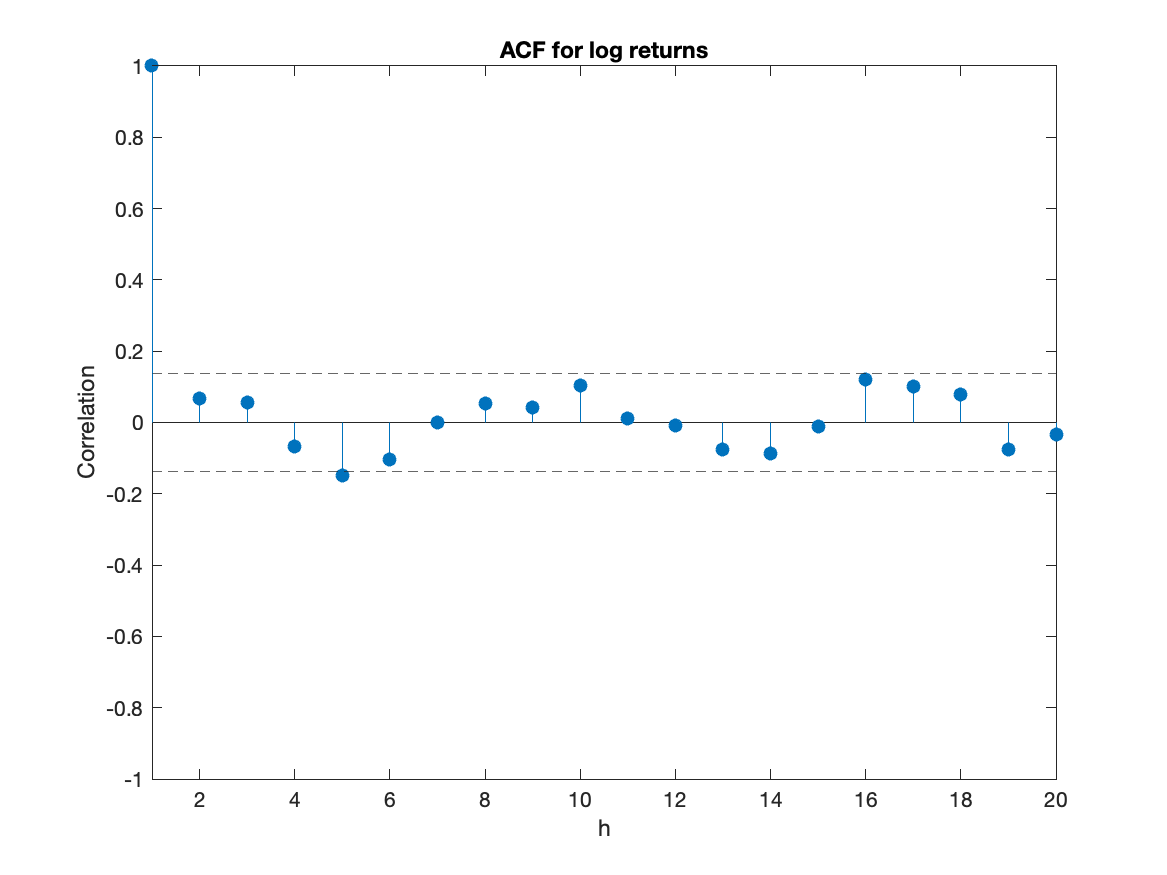
\includegraphics[width=10cm]{plots/acf_log_returns.png}
\centering
\caption{ACF for Log Returns $h = 0,\ldots, 20$}
\label{fig:acf_log}
\end{figure}

\section*{Problem 3}
We split the log returns into a training (first 102 observations) and the test set ($t = 103,\ldots, 204$).
Next we computed the autocovariance function $\hat{\gamma}$ using only the data from the training data set for each $h = 1,\ldots,20$.
$$
\hat{\gamma}(h) = \frac{1}{n} \sum_{t = 1}^{n - h}(X_{t + h} - \overline{X}) (X_t - \overline{X}) = \sum_{t = 1}^{n - h} X_{t + h} X_t
$$

We use these values in the sample covariance matrix
$$
\hat{\Gamma}_{20} = \begin{bmatrix}
    \hat{\gamma}(0)      & \hat{\gamma}(1) & \hat{\gamma}(2) & \dots & \hat{\gamma}(19) \\
    \hat{\gamma}(1)       & \hat{\gamma}(0) & \hat{\gamma}(0) & \dots & \hat{\gamma}(18) \\
    \vdots & \vdots & \vdots & \ddots & \vdots \\
    \hat{\gamma}(19)       & \hat{\gamma}(18) & \hat{\gamma}(17) & \dots & \hat{\gamma}(0)
\end{bmatrix}
$$
and solve for the coefficients, $a_1,\ldots, a_n$
$$
\hat{\Gamma}_{20} (a_1,\ldots, a_n)^T = (\hat{\gamma}(20), \hat{\gamma}(19),\ldots, \hat{\gamma}(1))^T
$$
Which results in the linear forecasts
\begin{align*}
b_n^l(z_{n-1}, \ldots, z_{n - 20}) &= a_1 z_{n - 1} + a_2 z_{n - 2} + \ldots + a_{20} z_{n - 20}\\
&= -0.098z_{n-1} + -0.018z_{n-2} + -0.179z_{n-3} + 0.101z_{n-4} + \\
&\qquad 0.015z_{n-5} + 0.088z_{n-6} + 0.115z_{n-7} + -0.097z_{n-8} +\\
&\qquad -0.036z_{n-9} + 0.061z_{n-10} + 0.013z_{n-11} + 0.096z_{n-12} +\\
&\qquad 0.098z_{n-13} + -0.048z_{n-14} + 0.051z_{n-15} + -0.035z_{n-16} +\\
&\qquad 0.005z_{n-17} + -0.158z_{n-18} + 0.062z_{n-19} + 0.192z_{n-20}
\end{align*}

In Figure \ref{fig:log_preds} we show the predictions in red and the actual values in black.
We can see as we go later in time the predictions tend towards the mean value of 0.

\begin{figure}[H]
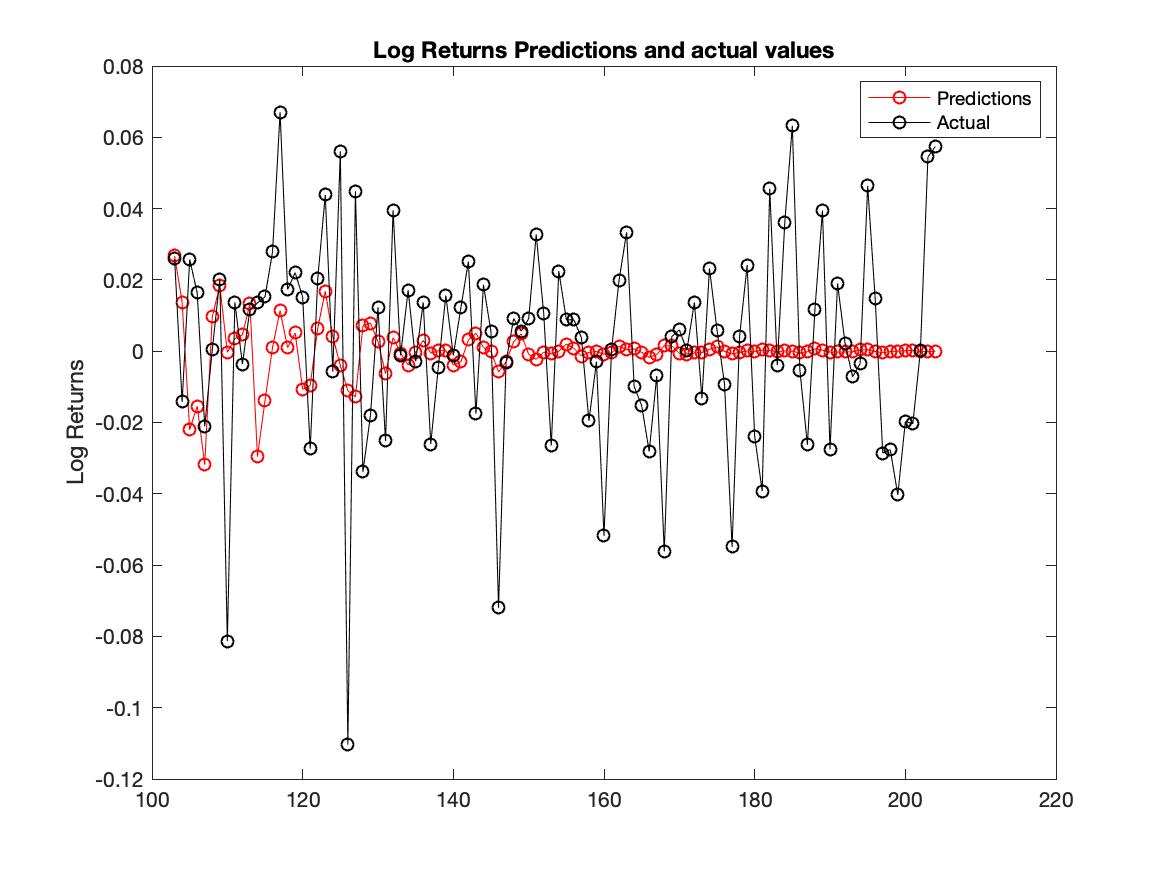
\includegraphics[width=10cm]{plots/log_returns_preds.png}
\centering
\caption{Linear predictions for $n = 103,\ldots, 204$}
\label{fig:log_preds}
\end{figure}

We computed the mean squared error
$$
\frac{1}{102} \sum_{n = 103}^{204} (b_n^l(z_{n-1}, \ldots, z_{n - 20}) - z_n)^2 = 0.00088
$$
where the prediction of just using the mean is
$$
\frac{1}{102} \sum_{103}^{204} z_n^2 = 0.00089
$$
We can see the the linear forecast MSE is almost exactly the same as the mean prediction.
We showed in problem 2 that the log returns looked iid.
This means that we have no correlation (besides noise) between the points in time.
We do not have any signal to predict from which results in the the linear forecasts being almost the same as the mean prediction.
We can see this behavior in Figure \ref{fig:log_preds} by noticiing that the predictions tend toward 0 as we go towards the end of the predictions.

\section*{Problem 4}
We created a QQ-plot, Figure \ref{fig:qqplot} for the log returns to check if the data was consistent with a normal distribution.
We sampled points from the standard normal distribution and compared against the order statistics for the normalized log returns.
We can see that the distribution of log returns does not look normal.

\begin{figure}[H]
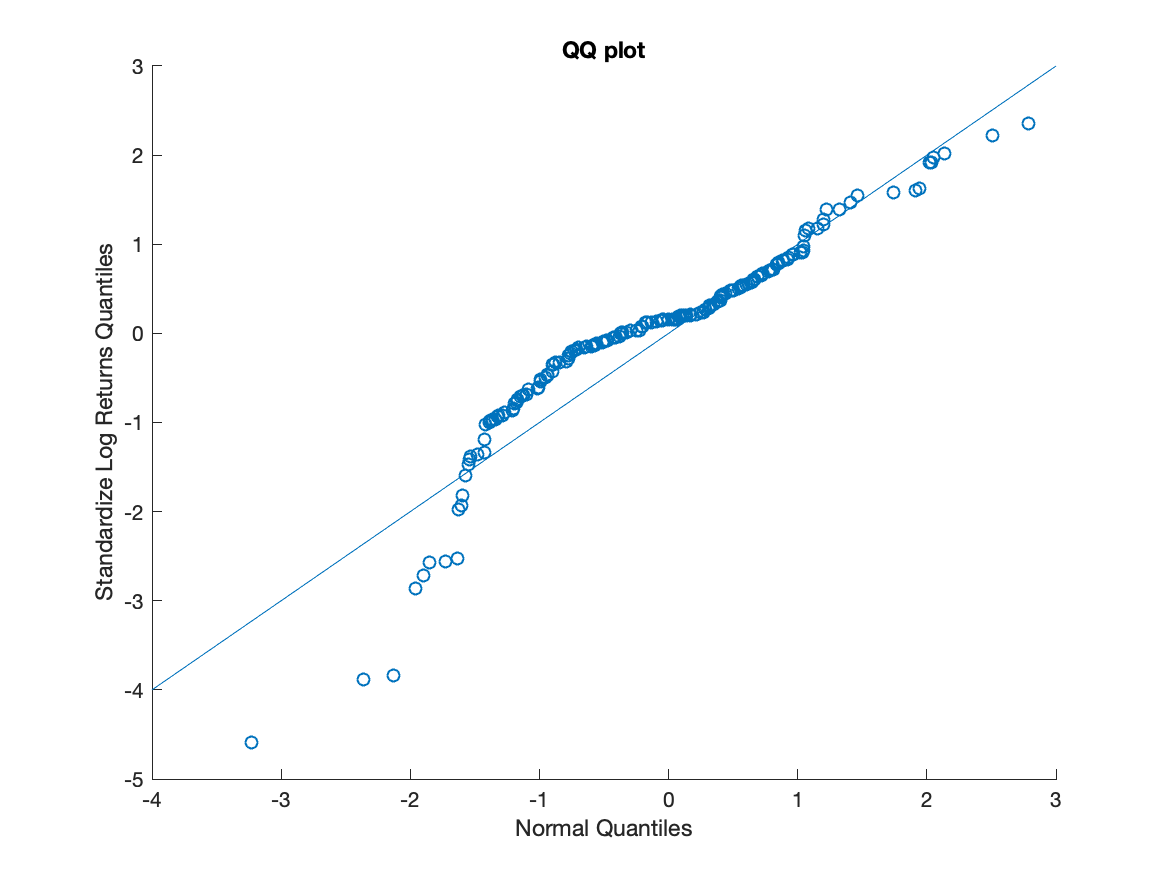
\includegraphics[width=10cm]{plots/qqplot.png}
\centering
\caption{QQ-plot for log returns}
\label{fig:qqplot}
\end{figure}

We then tested the series
$$
|Z_t| = |\log(X_{t + 1}) - \log(X_t)|
$$
using the Ljung-box test.
We found the critical value $\lambda_4 = 76.28 > 31.41$ so we can reject the null hypothesis that the absolute value of the returns are iid.
The p-value is $1.66 \times 10^{-8}$.

\section*{Problem 5}
\subsection*{Part a}
% Show expected value the same
\begin{align}
    E[X_t] &= E[\cos(\omega t + Y)] \nonumber\\
    &= E[\cos(\omega t) \cos(Y) - sin(\omega t) sin(Y)]  \label{ref1}\\
    &= \cos(\omega t) E[\cos(Y)] - sin(\omega t) E[sin(Y)] \nonumber\\
    &= \cos(\omega t) \cdot 0 - sin(\omega t) \cdot 0 = 0  \label{ref2}
\end{align}

\noindent \eqref{ref1} Trignonometric identity \\
\\
\eqref{ref2} 
\begin{align*}
E[\cos(Y)] &= \int_{-\infty}^{\infty} \cos(x) \mathbb{I}_{[-\pi, \pi]} dx \\
&= \int_{-\pi}^{\pi} cos(x) dx = [sin(x)]^{\pi}_{-\pi} = 0 + 0 = 0
\end{align*}

\begin{align*}
E[\sin(Y)] &= \int_{-\infty}^{\infty} \sin(x) \mathbb{I}_{[-\pi, \pi]} dx = \int_{-\pi}^{\pi} sin(x) dx\\ 
& = [-cos(x)]^{\pi}_{-\pi} = -\cos(\pi) - (- cos(-\pi)) \\
& = -(-1) - ( - (-1)) = 1 - 1 = 0
\end{align*}

\begin{align*}
\gamma_X(r,s) &= Cov(X_r, X_s) = E[cos(wr + Y)cos(ws + Y)] \\
 &= E[(\cos(wr)\cos(Y) - \sin(wr)\sin(Y))(\cos(ws)\cos(Y) - \sin(ws)\sin(Y)] \\
 &= E[\cos^2(Y)\cos(wr)\cos(ws) + \cos(wr)\cos(Y)\sin(wr)\sin(Y) - \sin(wr)\sin(Y)\cos(ws)\cos(Y) \\
 & + \sin^2(Y)sin(wr)sin(ws) ] \\
 & = E[\cos^2(Y)]\cos(wr)\cos(ws) + E[\cos(Y)\sin(Y)](\cos(wr)\sin(wr) - \sin(ws)\cos(ws)) \\
 & + E[\sin^2(Y)sin(wr)sin(ws)] \\
 & \underbrace{=}_{Additional \ calculation}  \pi (\cos(wr)\cos(ws) -\sin(wr)\sin(ws)) \\
 & \underbrace{=}_{trig. identity} \pi \cos(w(r-s)) \\
 & = \pi \cos(w((r + h) - (s + h)) \\
 & = \gamma_{X}(r+h, s+h)
 \end{align*}

This shows the process to be stationary.\\
\\
\\
\\
We can derive from the calculation of $Cov$ that for the Autocovariance holds the following:\\
$\gamma_X(h) = \pi \cos(wh)$
\\
\\
Additional Calculation:\\
In the first part we show $E[\cos^2(Y)] = \pi$ and $E[\sin^2(Y)] = \pi$. In the second part we show
$E[\sin(Y)\cos(Y)] = 0$

 
1) $ Y \sim \mathcal{U}[-\pi, \pi] $\\
\begin{align*}
 \int \cos^2(y) dy = & \int \cos(y)\cos(y) = \\
& \underbrace{=}_{Int. \ by \ parts} \sin(y)\cos(y) - \int -\sin(y)\sin(y) \\
& = \cos(y)\sin(y) + \int 1 - \cos^2(y) \\
& = \cos(y)\sin(y) + y + \int \cos^2(y) dy \\
&\Rightarrow 2\int \cos^2(y) dy = \cos(y)\sin(y) + y \\
&\Rightarrow \int \cos^2(y)dy = \frac 1 2 (\cos(y)\sin(y) + y) \\
\end{align*}
\begin{align*}
 \Rightarrow E[\cos^2(Y)] = \int_{-\pi}^{\pi} \cos^2(y)dy = [\frac 1 2 (\cos(y)\sin(y) + y) ]^{\pi}_{-\pi} = \pi
\end{align*}

\begin{align*}
E[\sin^2(Y)] = \dots = [\frac 1 2 (-\cos(y)\sin(y) + y) ]^{\pi}_{-\pi} = \pi
\end{align*}
2) $ Y \sim \mathcal{U}[-\pi, \pi] $
\begin{align*}
\int \sin(y)\cos(y)dy& \underbrace{=}_{u = \sin(y), \ du = cos(y)dy} \int u du \\
&= \frac 1 2 u^2 + C = \sin^2(y) + C \\
\end{align*}
\begin{align*}
\Rightarrow E[\sin(Y)\cos(Y)] = [\sin^2(y)]^{\pi}_{\pi} = 0 - 0 = 0
\end{align*}


\bibliographystyle{plain}
\bibliography{references}
\end{document}
